\documentclass[12pt]{article}
\usepackage{amsmath}
\usepackage{amsfonts}
\usepackage{parskip}
\usepackage{amsthm}
\usepackage{thmtools}
\usepackage[headheight=15pt]{geometry}
\geometry{a4paper, left=20mm, right=20mm, top=30mm, bottom=30mm}
\usepackage{graphicx}
\usepackage{bm} % for bold font in math mode - command is \bm{text}
\usepackage{enumitem}
\usepackage{fancyhdr}
\usepackage{amssymb} % for stacked arrows and other shit
\pagestyle{fancy}
\usepackage{changepage}
\usepackage{mathcomp}
\usepackage{tcolorbox}

\declaretheoremstyle[headfont=\normalfont]{normal}
\declaretheorem[style=normal]{Theorem}
\declaretheorem[style=normal]{Proposition}
\declaretheorem[style=normal]{Lemma}
\newcounter{ProofCounter}
\newcounter{ClaimCounter}[ProofCounter]
\newcounter{SubClaimCounter}[ClaimCounter]
\newenvironment{Proof}{\stepcounter{ProofCounter}\textsc{Proof.}}{\hfill$\square$}
\newenvironment{Solution}{\stepcounter{ProofCounter}\textbf{Solution:}}{\hfill$\square$}
\newenvironment{claim}[1]{\vspace{1mm}\stepcounter{ClaimCounter}\par\noindent\underline{\bf Claim \theClaimCounter:}\space#1}{}
\newenvironment{claimproof}[1]{\par\noindent\underline{Proof of claim \theClaimCounter:}\space#1}{\hfill $\blacksquare$ Claim \theClaimCounter}
\newenvironment{subclaim}[1]{\stepcounter{SubClaimCounter}\par\noindent\emph{Subclaim \theClaimCounter.\theSubClaimCounter:}\space#1}{}
% \newenvironment{subclaimproof}[1]{\begin{adjustwidth}{2em}{0pt}\par\noindent\emph{Proof of subclaim \theClaimCounter.\theSubClaimCounter:}\space#1}{\hfill
% $\blacksquare$ \emph{Subclaim \theClaimCounter.\theSubClaimCounter}\vspace{5mm}\end{adjustwidth}}
\newenvironment{subclaimproof}[1]{\par\noindent\emph{Proof of subclaim \theClaimCounter.\theSubClaimCounter:}\space#1}{\hfill
$\Diamond$ \emph{Subclaim \theClaimCounter.\theSubClaimCounter}}

\allowdisplaybreaks{}

% chktex-file 3

\title{STAT 520: Exam 2}
\author{Evan P. Walsh}
\makeatletter
\makeatother
\lhead{Evan P. Walsh}
\chead{STAT 520: Exam 2}
\rhead{\thepage}
\cfoot{}

\begin{document}
% \maketitle

\section*{Tornados}

\begin{enumerate}[leftmargin=*]
  \item \textbf{A simple model.}
    \begin{enumerate}[leftmargin=1mm]
      \item Let $\bm{Y} = Y_1, \dots, Y_n$, where $n = 47$, be random variables associated with the number of tornados in each of the 47 states we are
        interested in. Since the data are discrete and non-negative, it is natural to consider a Poisson data model with a gamma conjugate prior.
        We will treat these random variables as independent and, for now, identically distributed. Thus,
        the joint pdf of the data model will have the form
        \[
          f(\bm{y}|\lambda) = \prod_{i=1}^{n} e^{-\lambda}\lambda^{y_i} \frac{1}{y_i!} = e^{-n\lambda}\lambda^{n\bar{y}}
          \prod_{i=1}^{n}\frac{1}{y_i!},
        \]
        where $\lambda$ is the average number of tornados per state, and the prior pdf of $\lambda$ will have the form
        \[
          \pi(\lambda) = \beta_0^{\alpha_0} \lambda^{\alpha_0 - 1}\exp\{-\beta_0\lambda\} \frac{1}{\Gamma(\alpha_0)},
        \]
        for some known $\alpha_0, \beta_0 > 0$.

      \item Based on our model formulation in part (a),
        \[
          p(\lambda|\bm{y}) \propto f(\bm{y}|\lambda) \pi(\lambda) \propto \exp\{-(n + \beta_0)\lambda\} \lambda^{(n\bar{y} + \alpha_0) - 1},
        \]
        which is the kernel of a gamma distribution with shape parameter $\alpha = n\bar{y} + \alpha_0$ and rate parameter $\beta = n + \beta_0$.

      \item In order for the prior to have an expectation of 5 and variance of 10, we must set $\alpha_0 := 2.5$ and $\beta_0 := 0.5$. A summary of
        the resulting posterior distribution for $\lambda$ is given below in Table \ref{tab:1}.

        \begin{table}[h!]
          \centering
          \begin{tabular}{lc}
            \hline
            Posterior shape $\alpha$ & 975.5 \\
            \hline
            Posterior rate $\beta$ & 47.5  \\
            \hline
            Posterior expectation & 20.537 \\
            \hline
            90\% credible interval for $\lambda$ & (19.467, 21.630) \\
            \hline
          \end{tabular}
          \caption{Summary of the posterior distribution for $\lambda$.}
          \label{tab:1}
        \end{table}

      \item We conducted a posterior predictive assessment of this model with $M = 10,000$ iterations 
        using the data characteristics of (1) the number of states with at least 50
        tornados ($Q_1(\bm{y})$) and (2) the range in the number of tornados across all states ($Q_2(\bm{y})$). The posterior predictive p-value for
        both $Q_1(\bm{y})$ and $Q_2(\bm{y})$ were 0, which indicates that our model is drastically inadequate.

    \end{enumerate}

    \newpage
  \item \textbf{A second model.}
    \begin{enumerate}[leftmargin=1mm]
      \item Let $K_i$ represent the size of the $i^{th}$ state in units of 1000 square kilometers. We now formulate a Poission data model where the 
        expected number of tornados in state $i$ is given by $\rho K_i$, where $\rho > 0$ is a ``rate'' parameter\footnote{Not to be confused with the
        rate parameter of a gamma distribution.} which represents the average number of tornados per 1000 $km^2$.
        We assume independence once again.
        Therefore the joint pdf of data model is given by 
        \[
          f(\bm{y}|\rho) = \prod_{i=1}^{n} e^{-\rho K_i}(\rho K_i)^{y_i} \frac{1}{y_i!} = e^{-\rho n\bar{y}}\rho^{n\bar{y}}
          \prod_{i=1}^{n}\frac{K_i^{y_i}}{y_i!},
        \]

      \item Using the same prior as in question 1, but this time for the rate parameter $\rho$, we have 
        \[
          \pi(\rho) = \beta_0^{\alpha_0}\rho^{\alpha_0 - 1}\exp\{-\beta_0\rho\} \frac{1}{\Gamma(\alpha_0)},
        \]
        and so
        \[
          p(\rho|\bm{y}) \propto \exp\left\{-\left(\sum K_i + \beta_0\right)\rho\right\} \rho^{(n\bar{y} + \alpha_0) - 1},
        \]
        which is the kernel of a gamma distribution with shape $\alpha = n\bar{y} + \alpha_0$ and rate $\beta = \sum K_i + \beta_0$.
        Hence our model choice has led to a conjugate prior once again.

      \item A summary of the posterior distribution for $\rho$ using the same prior parameters as in part 1 (c) is given below in Table \ref{tab:2}.

        \begin{table}[h!]
          \centering
          \begin{tabular}{lc}
            \hline
            Posterior shape $\alpha$ & 975.5 \\
            \hline
            Posterior rate $\beta$ & 6992.4  \\
            \hline
            Posterior expectation & 0.1395 \\
            \hline
            90\% credible interval for $\rho$ & (0.1322, 0.1469) \\
            \hline
          \end{tabular}
          \caption{Summary of the posterior distribution for $\rho$.}
          \label{tab:2}
        \end{table}

      \item We conducted a posterior predictive assessment of this model with $M = 10,000$ iterations 
        using the the same characteristics $Q_1$ and $Q_2$ of part 1 (d). The posterior predictive p-value for
        $Q_1(\bm{y})$ was $0.0032$ and for $Q_2(\bm{y})$ was $0.0047$, which indicates that the new model is a slight improvement over the model from
        part 1, yet is still inadequate according to these criteria.

    \end{enumerate}

  \item \textbf{A final model.}

    \begin{enumerate}[leftmargin=1mm]
      \item We now modify the model from part 2 to consist of two groups, $\bm{Y}_1$ and $\bm{Y}_2$, where group 1 consists of the states
        within Tornado Alley and Dixie Alley, and group 2 consists of the remaining states (out of the 47) that are not in group 1.
        Let $n_1$ and $n_2$ be the number of states in group 1 and group 2, respectively. For $j = 1,2$, the pdf of the data model of group $j$ is 
        \[
          f(\bm{y}|\rho_j) = \prod_{i=1}^{n_j} e^{-\rho_j K_i}(\rho_j K_i)^{y_i} \frac{1}{y_i!} = e^{-\rho_j n_j\bar{y}}\rho_j^{n\bar{y}}
          \prod_{i=1}^{n_j}\frac{K_i^{y_i}}{y_i!}.
        \]

      \item For $\rho_1$ and $\rho_2$ we use the same form of the prior given in part 2 (b), yet with $\alpha_0 = \beta_0 = 0.1$ so that the prior
        expectation is 1 and the variance is 10. A summary of the posterior distribution of $\rho_j$ for each group is shown below in Table
        \ref{tab:3}.

        \begin{table}[h!]
          \centering
          \begin{tabular}{lcc}
            & Group 1 & Group 2 \\
            \hline
            Posterior shape $\alpha$ & 363.1 & 610.1 \\
            \hline
            Posterior rate $\beta$ & 1286.0 & 5706.1  \\
            \hline
            Posterior expectation & 0.2824 & 0.1069 \\
            \hline
            90\% credible interval for $\rho_j$ & (0.2584, 0.3072) & (0.0999, 0.1141) \\
            \hline
          \end{tabular}
          \caption{Summary of the posterior distribution for the rate parameter $\rho_j$ of each group.}
          \label{tab:3}
        \end{table}

      \item If we treat the posterior distributions as independent, then we can compute the probability that $\rho_1 > \rho_2$ as
        \begin{align}
          P(\rho_1 > \rho_2) & = \int_{0}^{\infty}\int_{0}^{\rho_1}p(\rho_1|\bm{y}_1)p(\rho_2|\bm{y}_2) d\mu(\rho_2)d\mu(\rho_1) \nonumber \\
          & = \int_{0}^{\infty} F_{2}(\rho_1)p(\rho_1|\bm{y}_1) d\mu(\rho_1) \label{eq:1}
        \end{align}
        where $F_{2}(\rho_1)$ is the posterior cdf of $\rho_2$ evaluated at $\rho_1$.
        It should be obvious from Figure \ref{fig:1} that this probability is extremely close to 1. To be thorough, however, we estimated the integral
        in \eqref{eq:1}
        numerically using a 
        Monte-Carlo simulation with a Monte-Carlo sample size of $M = 10,000$. 
        In particular, we simulated 10,000 random variables $\{x_{m}^{*}\}_{m=1}^{M}$ from the distribution given by $p(\rho_1|\bm{y}_1)$ and 
        then calculated the sample mean of $\{F_{2}(x_{m}^{*})\}_{m=1}^{M}$. The resulting estimate was indeed 1. Thus,
        \[
          P(\rho_1 > \rho_2) \approx 1.
        \]
        % \begin{align}
          % P(\rho_1 > \rho_2) & = \int_{0}^{\infty}\int_{0}^{\rho_1}p(\rho_1|\bm{y}_1)p(\rho_2|\bm{y}_2) d\mu(\rho_2)d\mu(\rho_1) \nonumber \\
          % & = \int_{0}^{\infty} \int_{0}^{\rho_1} \frac{\rho_1^{\alpha_1 - 1}\exp\{-\beta_1 \rho_1\}\rho_2^{\alpha_2 - 1}\exp\{-\beta_2 \rho_2\}}{
          % \beta_1^{-\alpha_1} \Gamma(\alpha_1) \beta_2^{-\alpha_2} \Gamma(\alpha_2)} d\mu(\rho_2)d\mu(\rho_1) \nonumber \\
          % & = \frac{\beta_1^{\alpha_1} \beta_2^{\alpha_2}}{\Gamma(\alpha_1)\Gamma(\alpha_2)} \int_{0}^{\infty} \int_{0}^{\rho_1} 
          % \rho_1^{\alpha_1 - 1}\exp\{-\beta_1 \rho_1\}\rho_2^{\alpha_2 - 1}\exp\{-\beta_2 \rho_2\} d\mu(\rho_2)d\mu(\rho_1),
          % \label{eq:1}
        % \end{align}
        % where $(\alpha_1, \beta_1), (\alpha_2, \beta_2)$ are the parameters of the posterior distribution for $\rho_1$ and $\rho_2$, respectively, 
        % as given in Table \ref{tab:3}.
        % In order to evaluate the integral in \eqref{eq:1}, 

      \item We conducted a posterior predictive assessment of this model with $M = 10,000$ iterations 
        using the same characteristics $Q_1$ and $Q_2$ of part 1 (d) for each group. For group 1, the posterior predictive p-values 
        were $0.3528$ and $0.0684$ for $Q_1$ and $Q_2$, respectively, while for group 2, the posterior predictive p-values were
        $0.0195$ and $0.0065$ for $Q_1$ and $Q_2$, respectively. This suggests that the model may be adequate according to the first criteria $Q_1$,
        although the p-value for group 2 is fairly small, but
        is still definitely inadequate according to the second criteria $Q_2$.

      \item Below is a plot of the posterior distributions of $\rho_j$ for each group.

        \begin{figure}[h!]
          \centering
          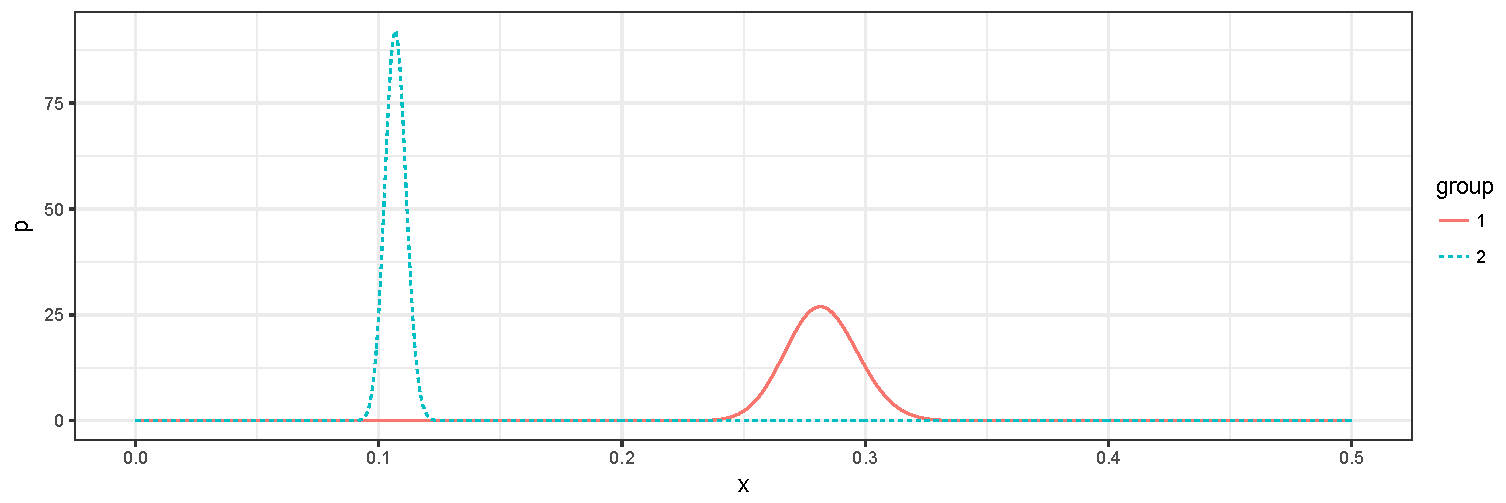
\includegraphics[width=0.9\textwidth]{./figures/exam02.pdf}
          \caption{Posterior distributions of the rate parameter $\rho_j$ for each group.}
          \label{fig:1}
        \end{figure}
    \end{enumerate}
\end{enumerate}


\end{document}
